\newcommand{\mapwidth}{0.32\textwidth}

\begin{figure}[htbp]
    \centering
    
    % Row 1
    \begin{subfigure}[b]{\mapwidth}
        \centering
        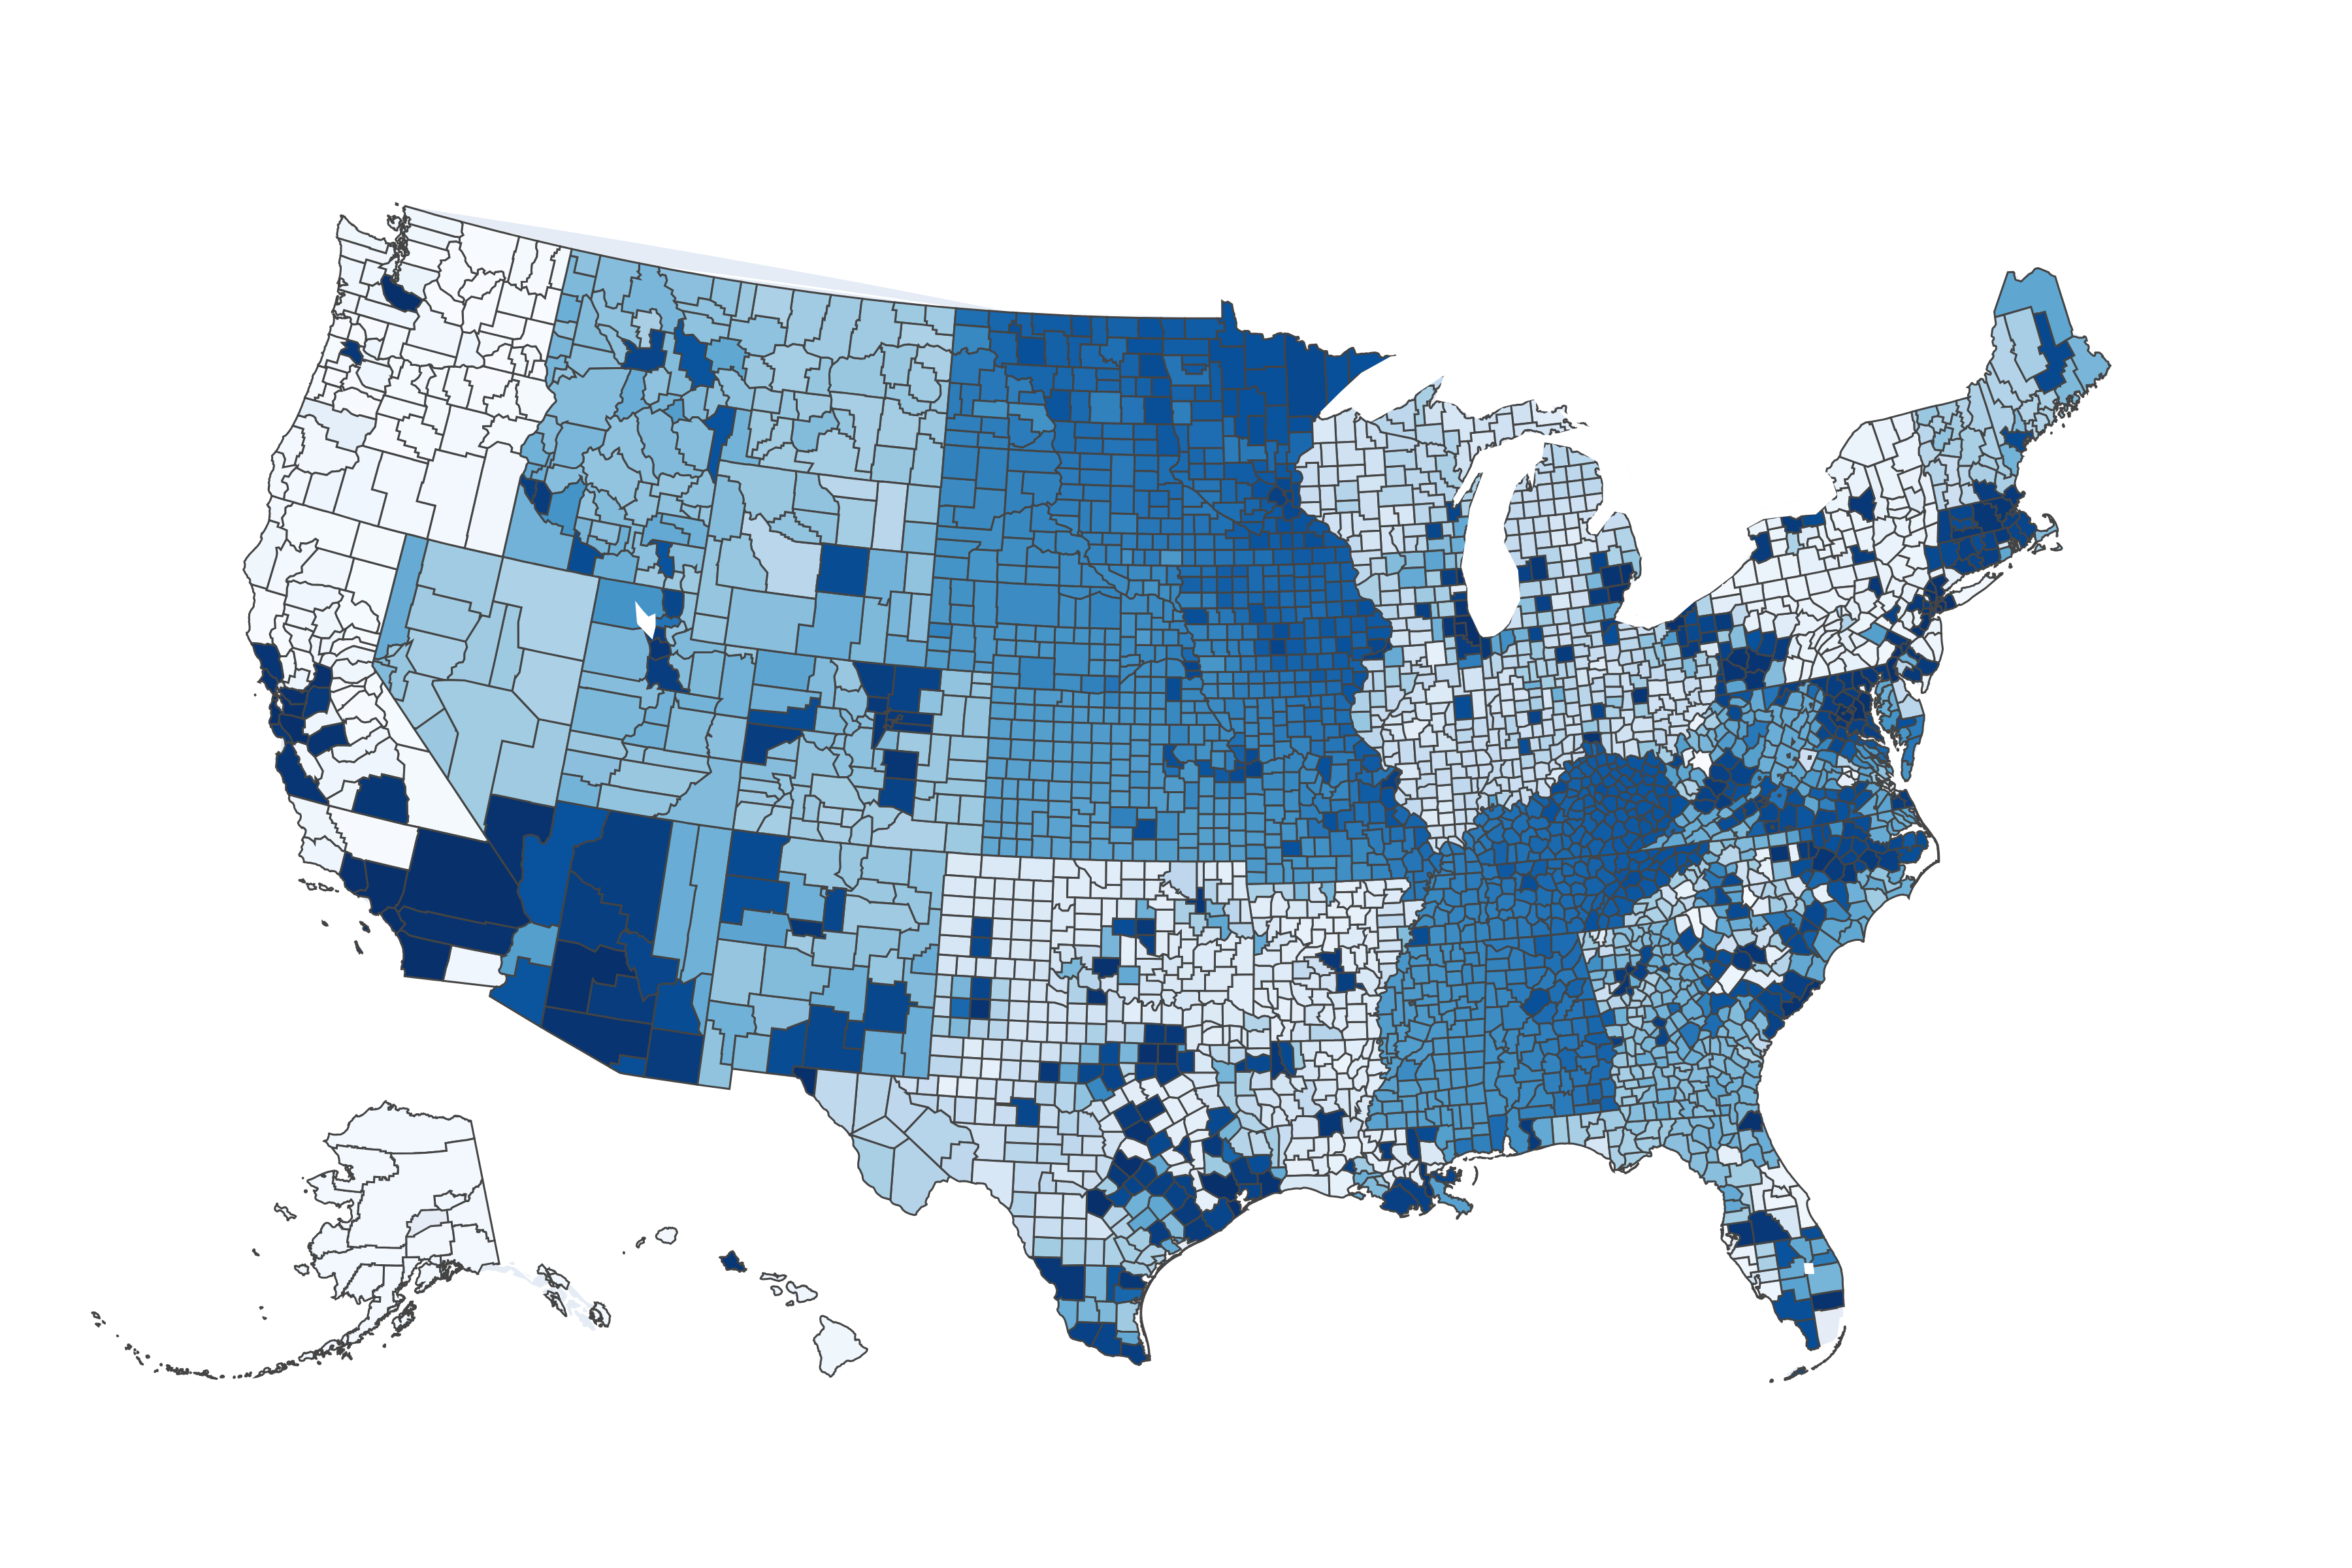
\includegraphics[width=\textwidth]{figures/maps/immigration_shock_1980.png}
        \caption*{\small 1975-1980}
    \end{subfigure}
    \hfill
    \begin{subfigure}[b]{\mapwidth}
        \centering
        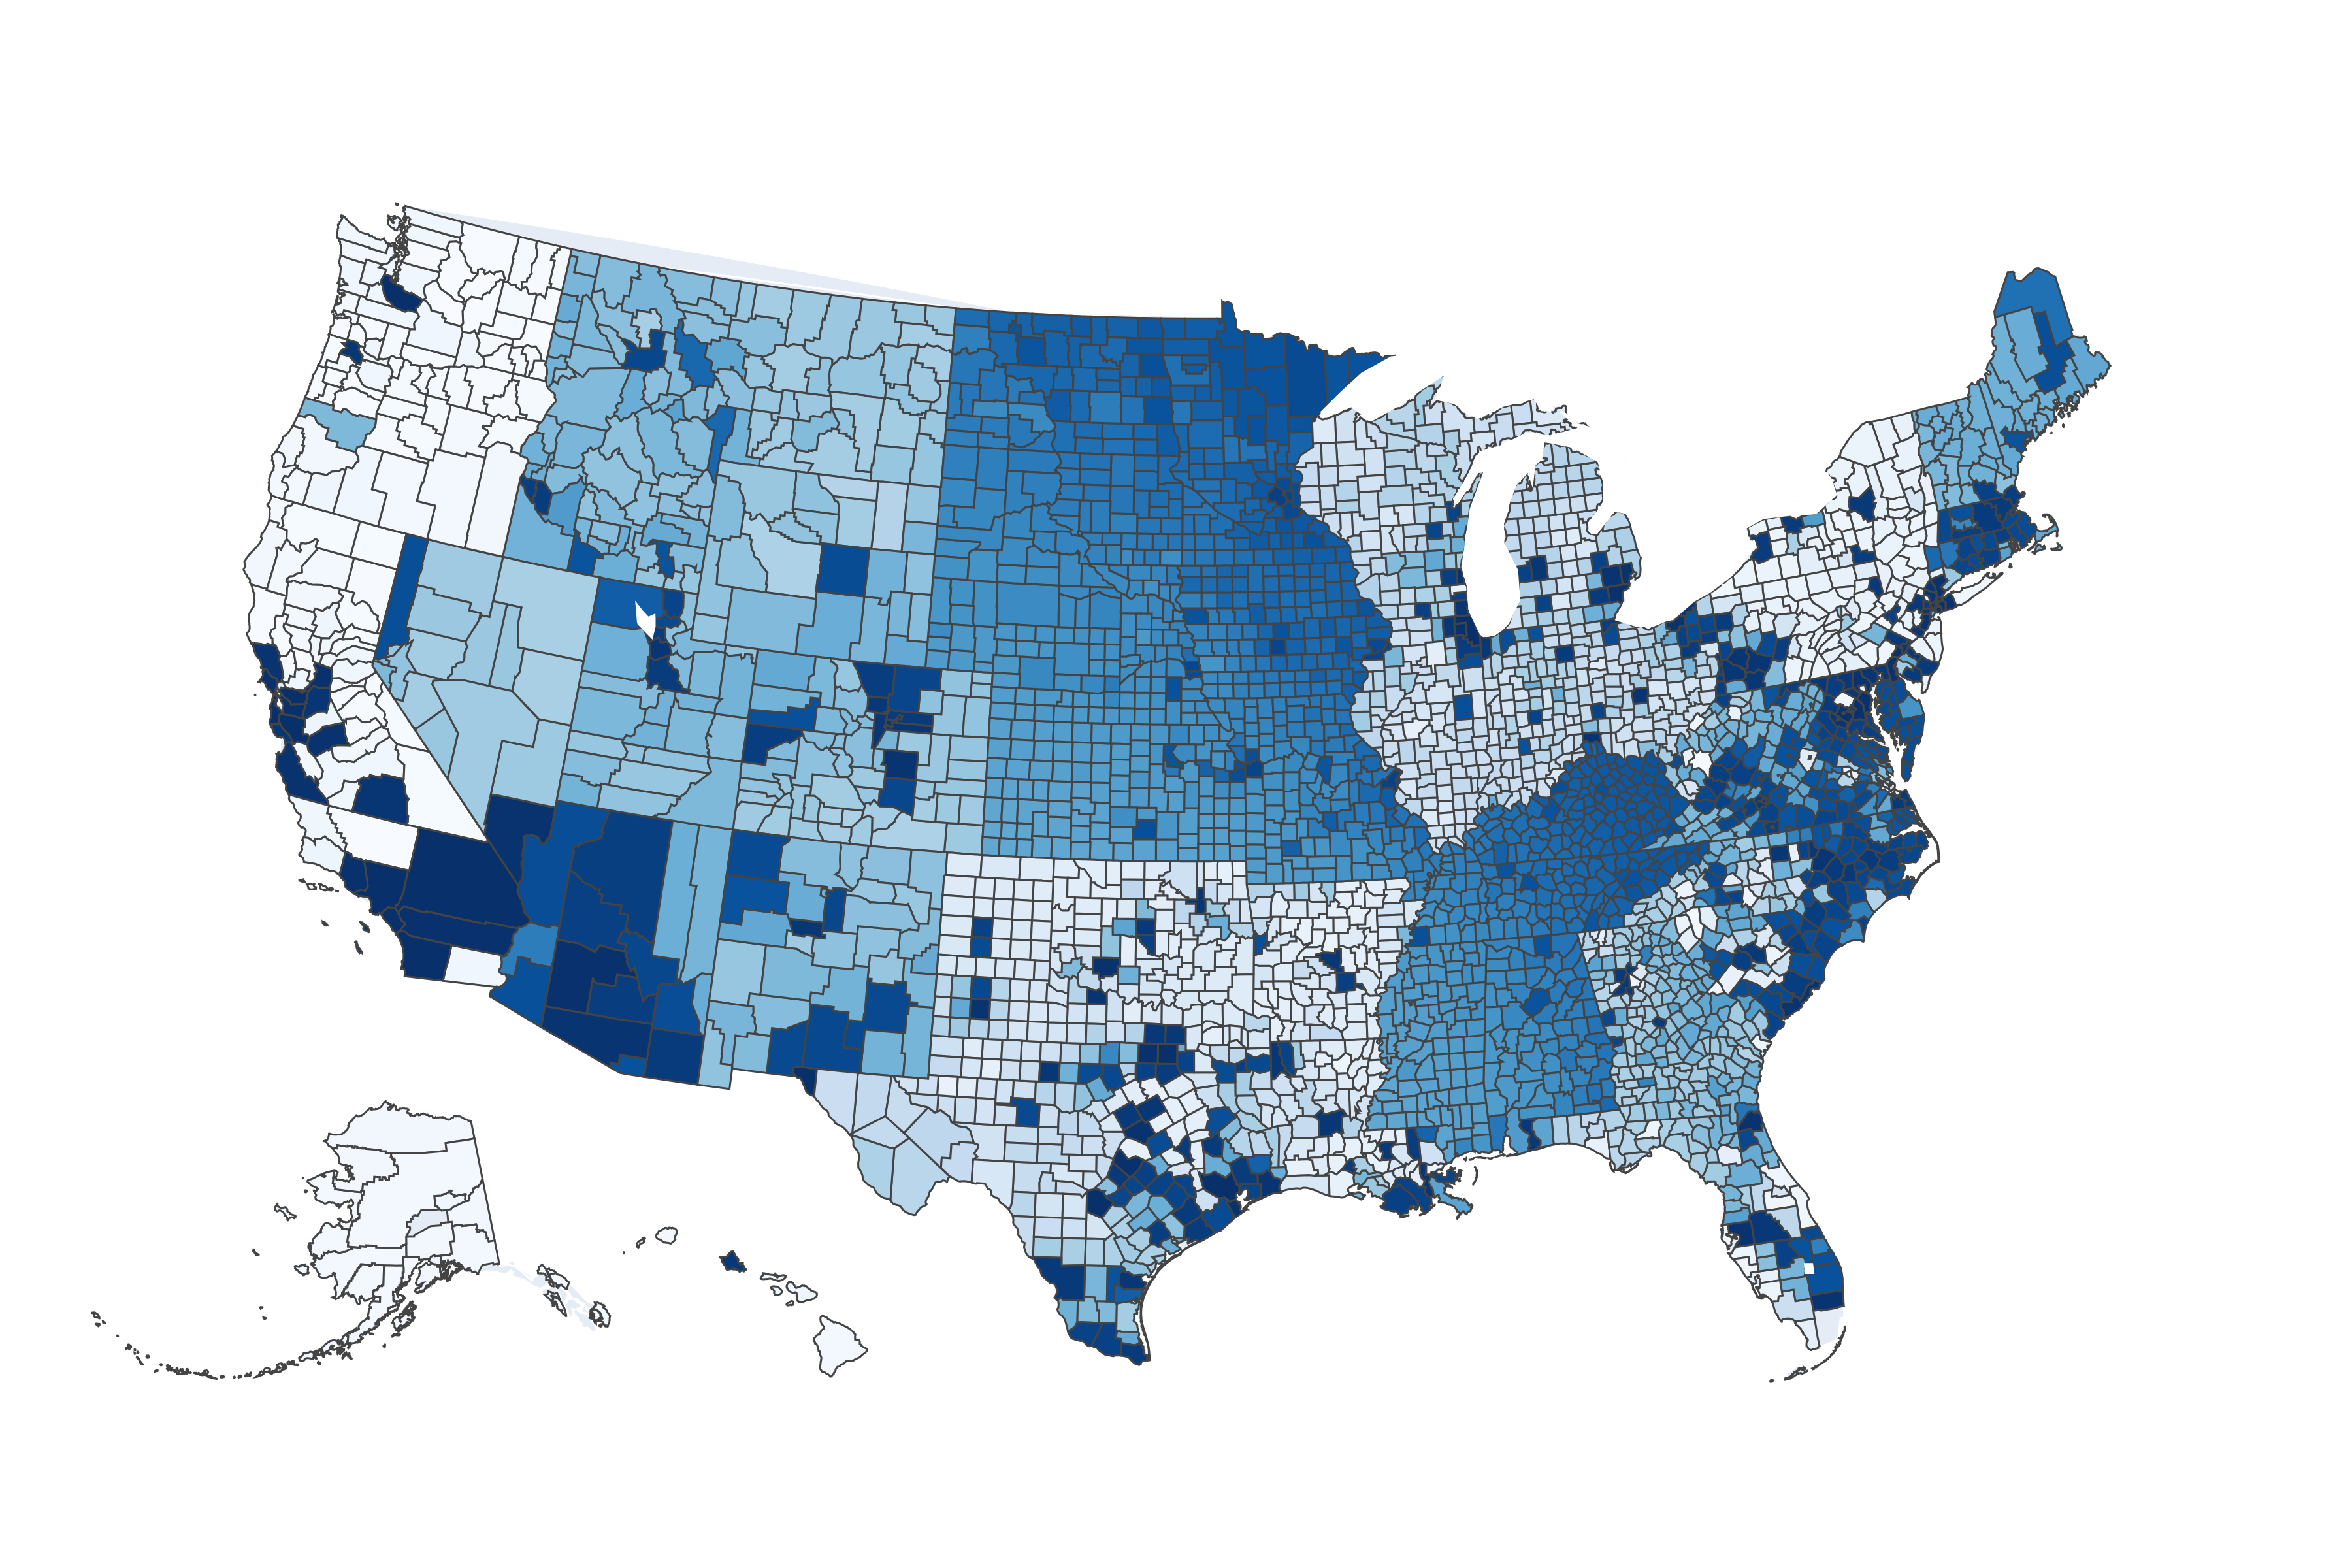
\includegraphics[width=\textwidth]{figures/maps/immigration_shock_1985.png}
        \caption*{\small 1980 - 1985}
    \end{subfigure}
    \hfill
    \begin{subfigure}[b]{\mapwidth}
        \centering
        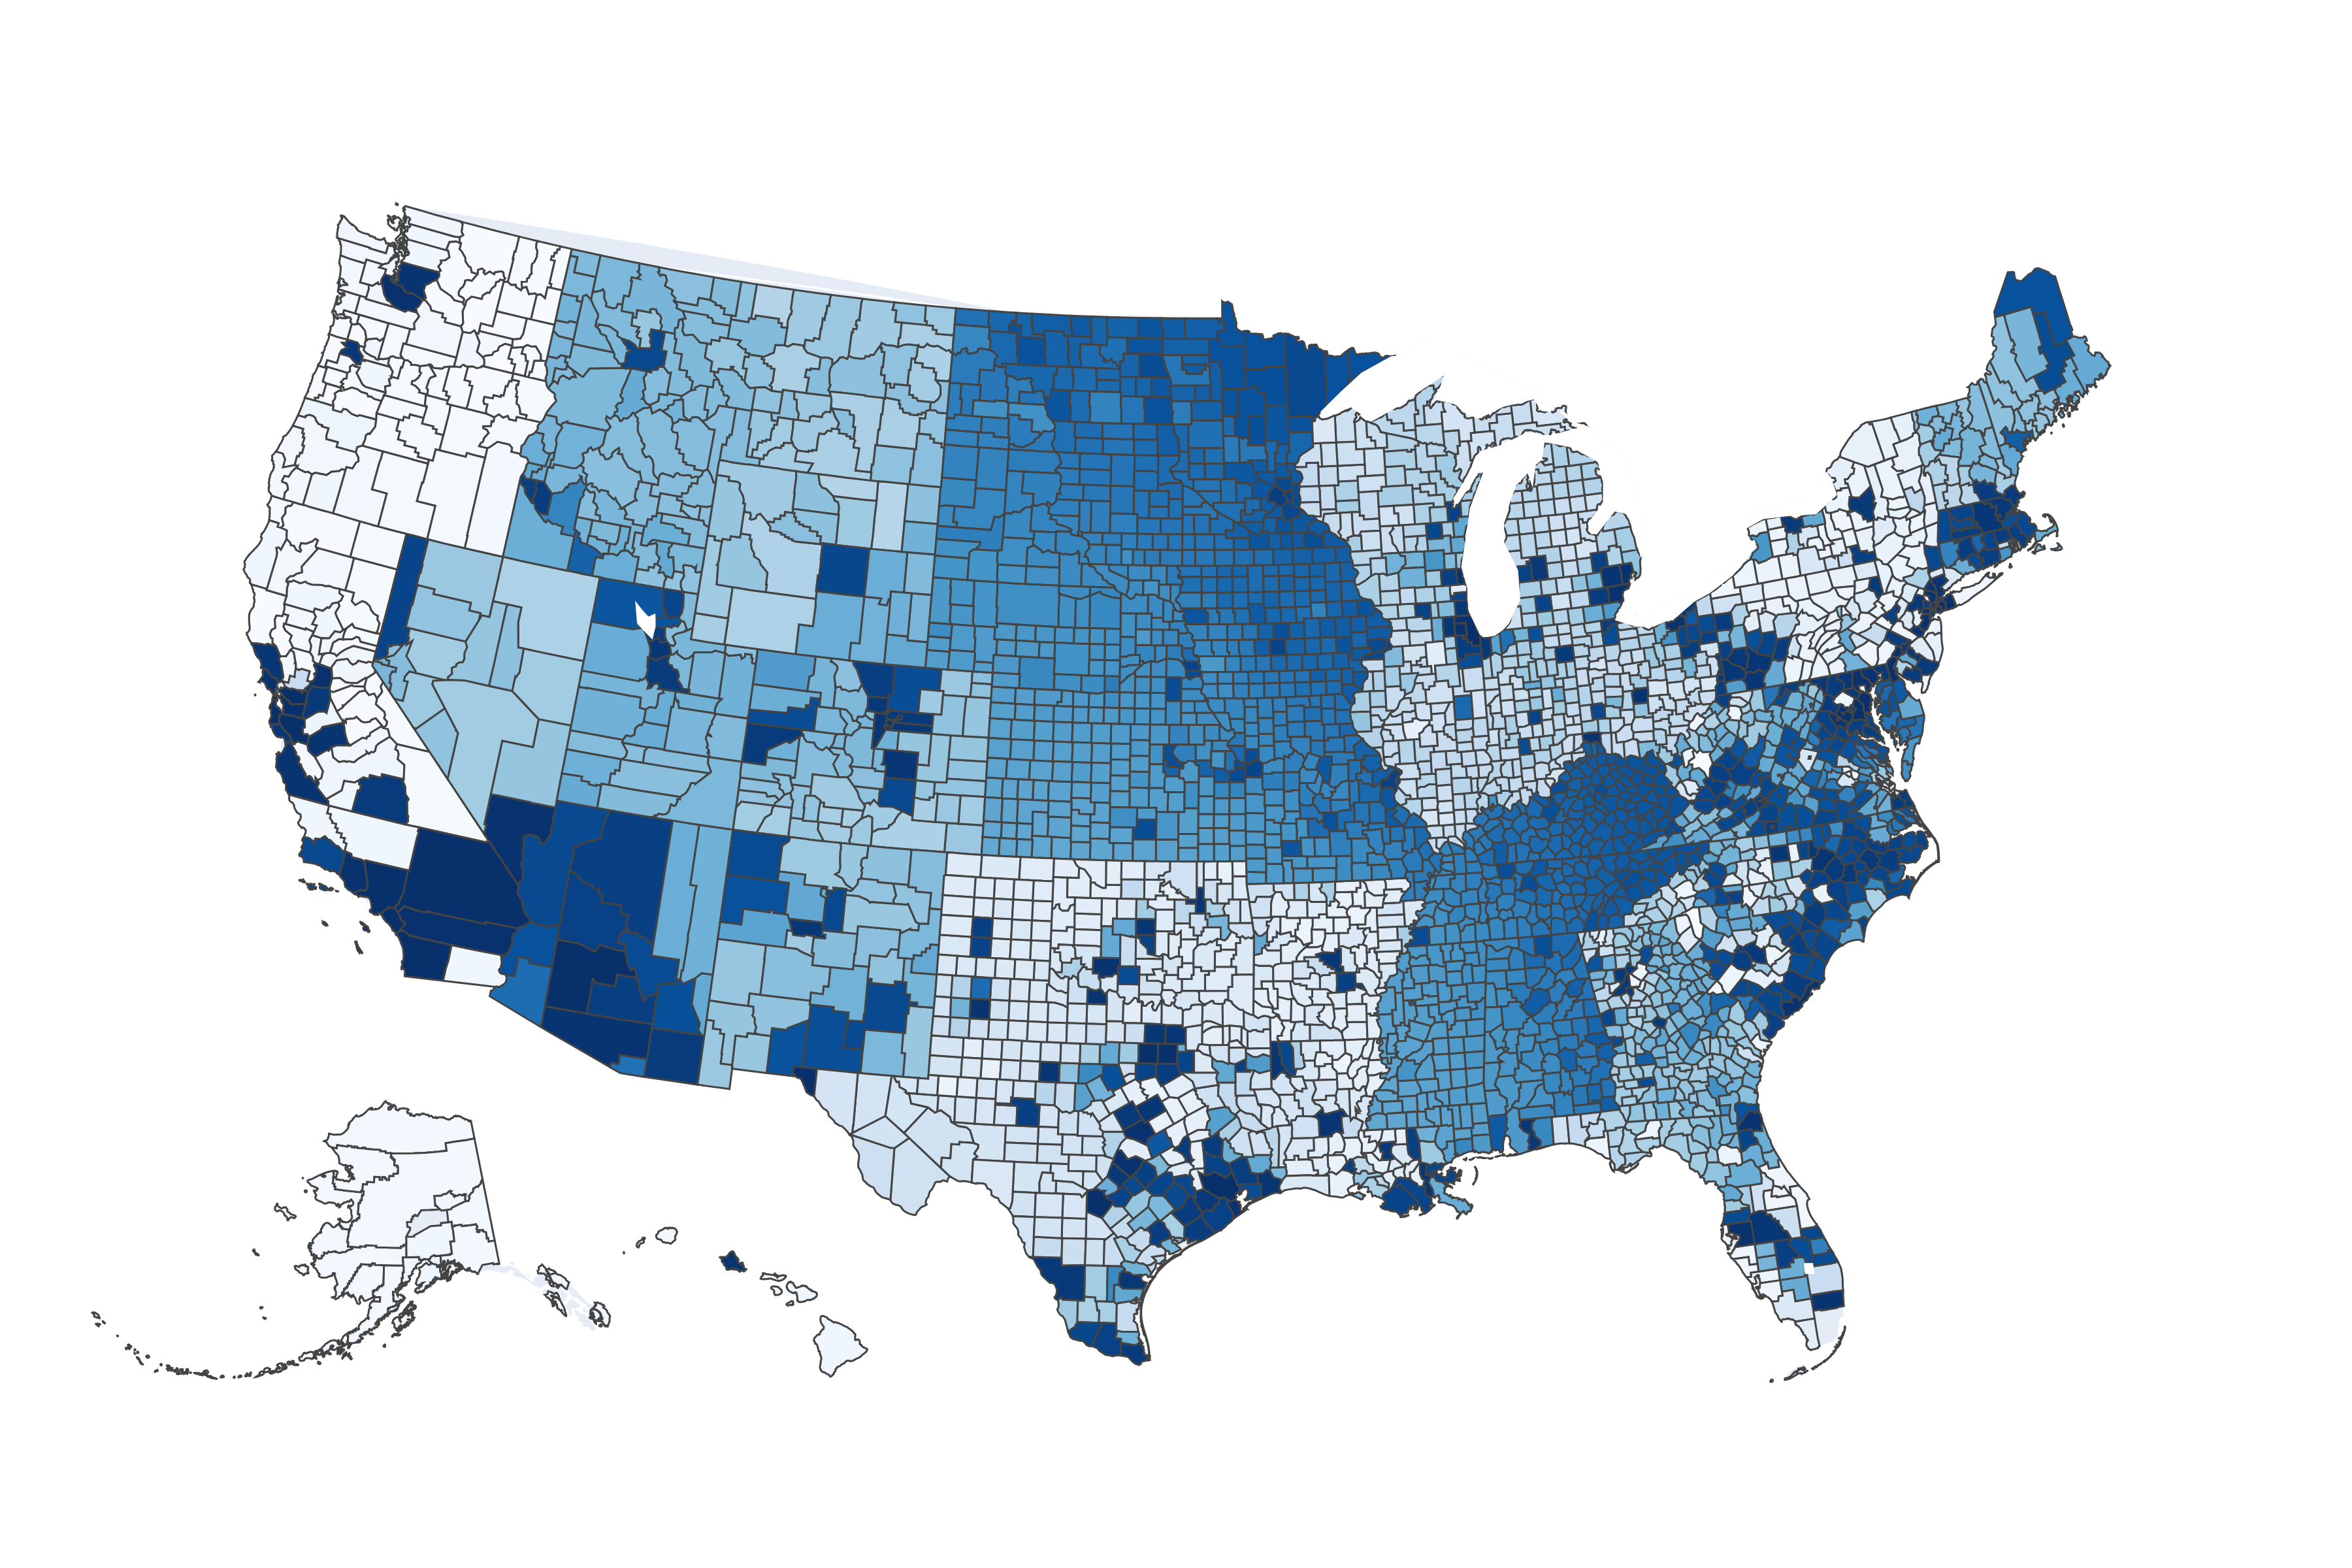
\includegraphics[width=\textwidth]{figures/maps/immigration_shock_1990.png}
        \caption*{\small 1985 - 1990}
    \end{subfigure}
    
    \vspace{0.3em}
    
    % Row 2
    \begin{subfigure}[b]{\mapwidth}
        \centering
        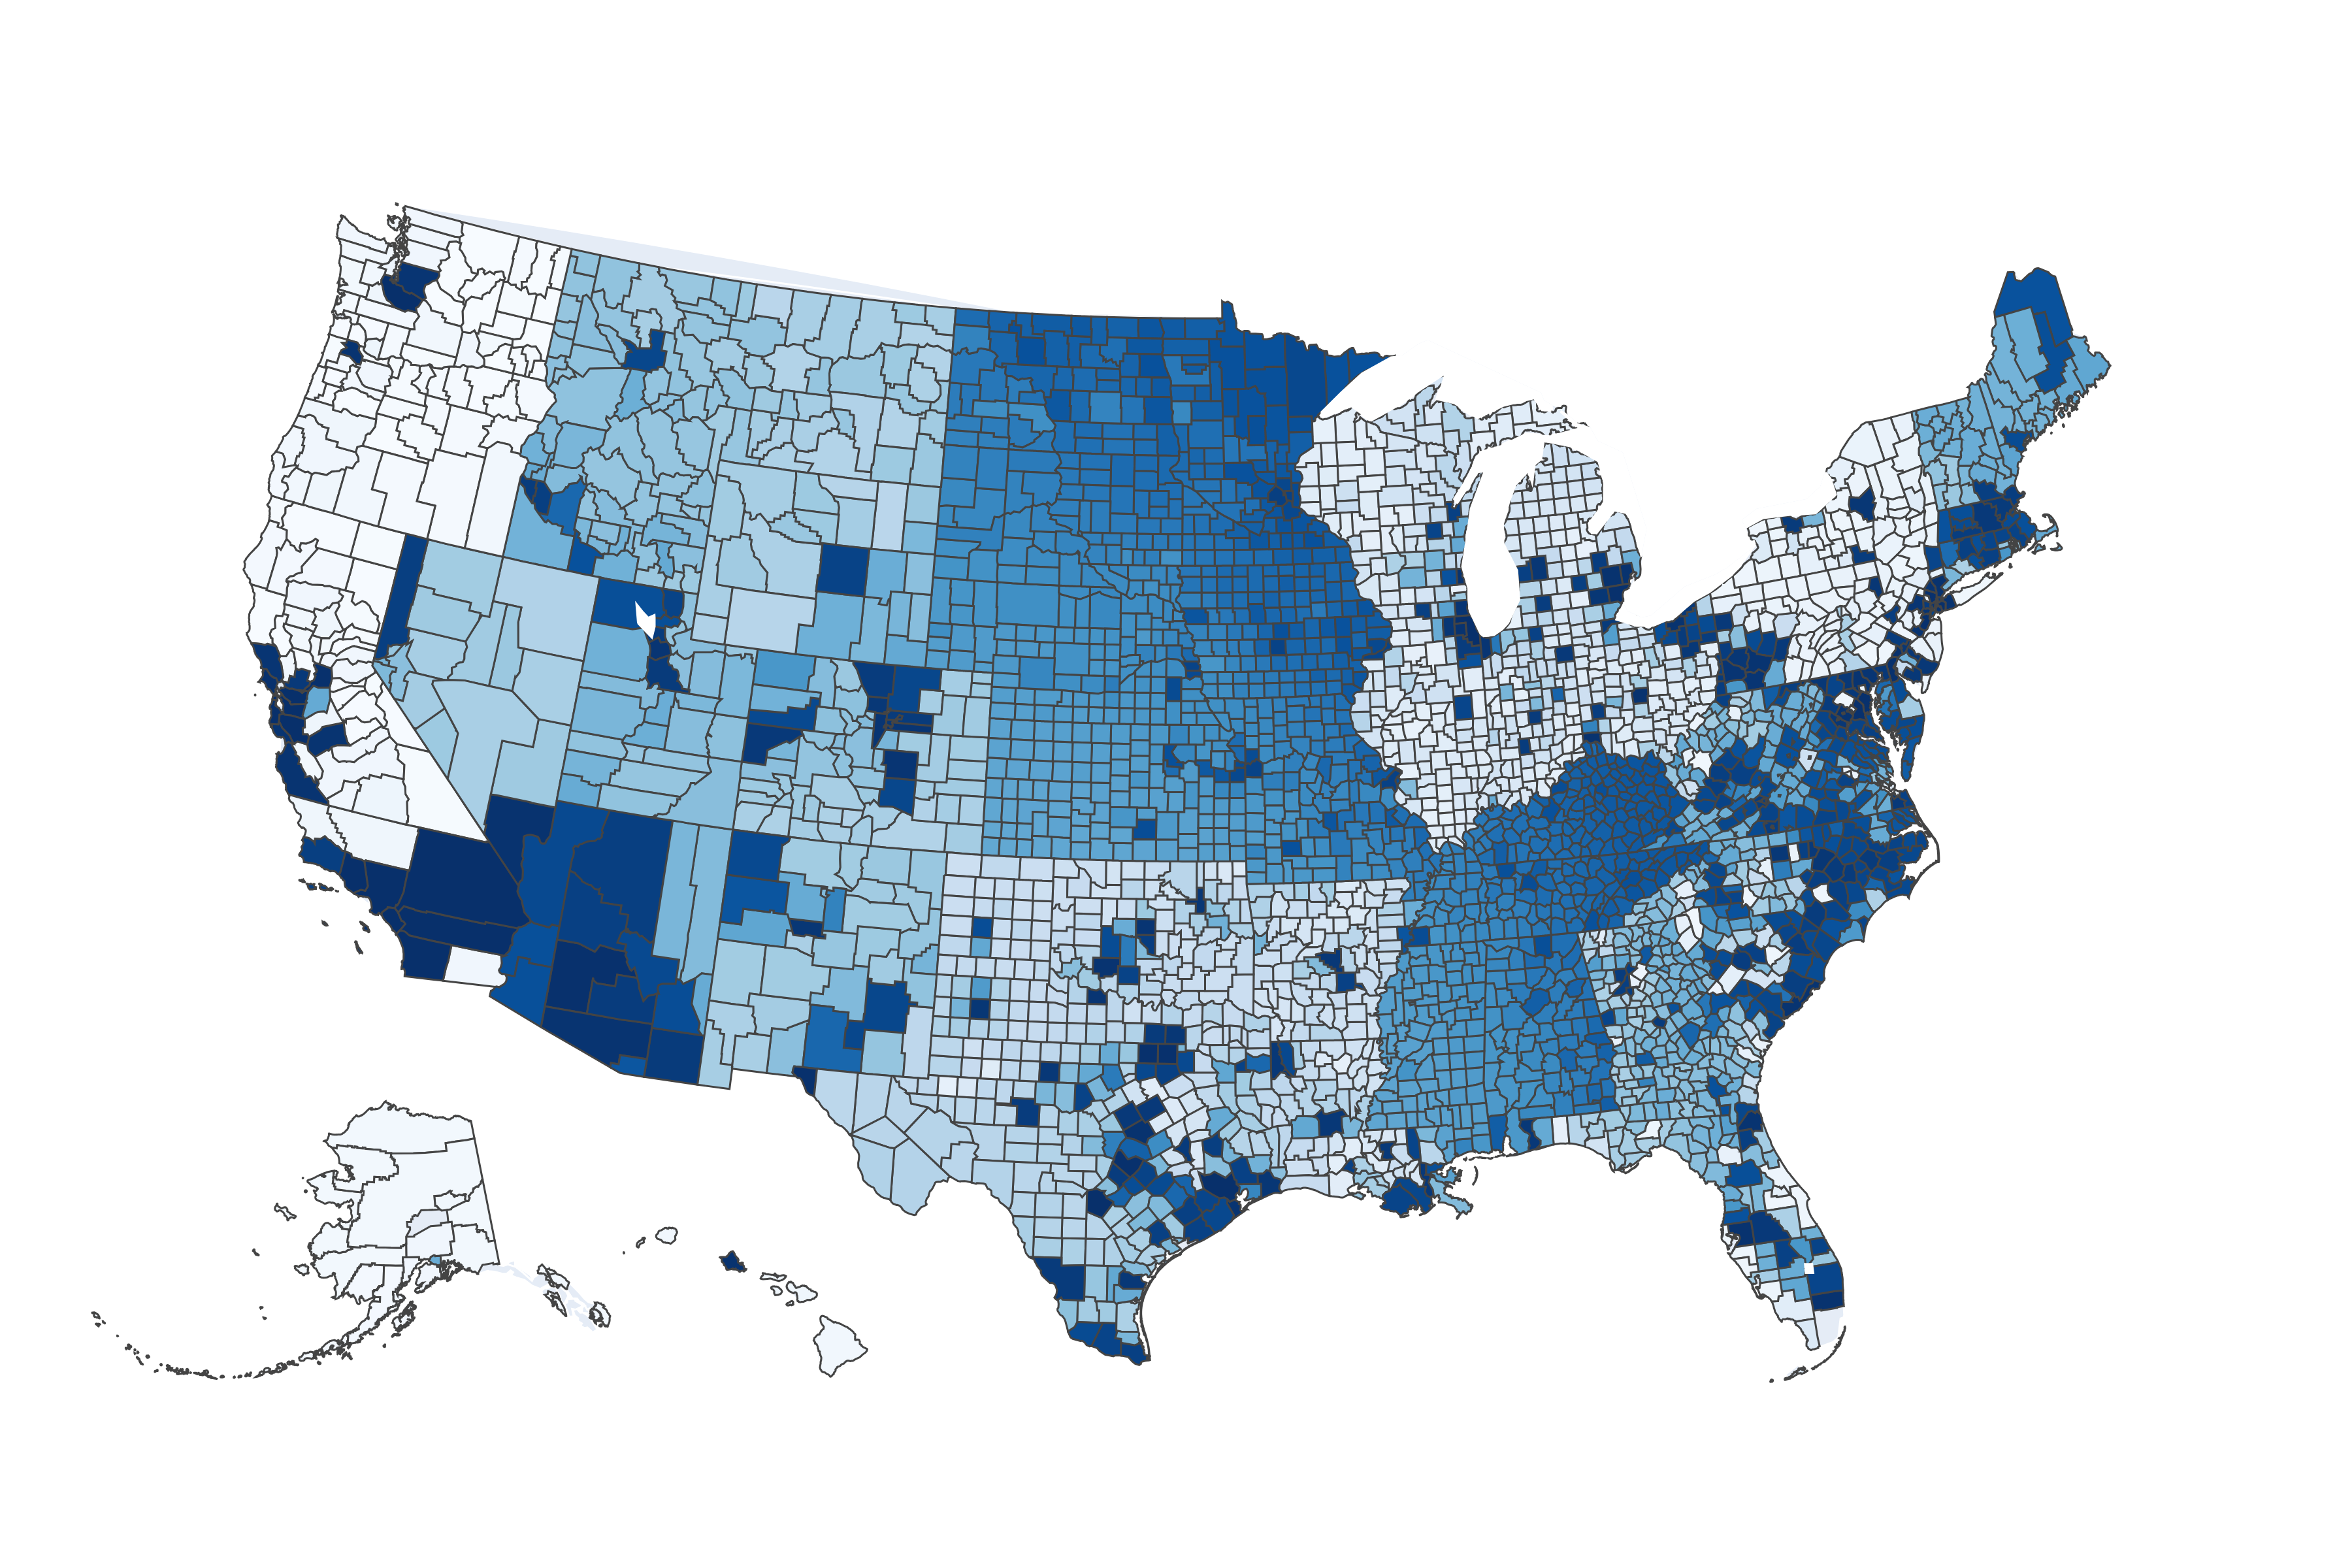
\includegraphics[width=\textwidth]{figures/maps/immigration_shock_1995.png}
        \caption*{\small 1990 - 1995}
    \end{subfigure}
    \hfill
    \begin{subfigure}[b]{\mapwidth}
        \centering
        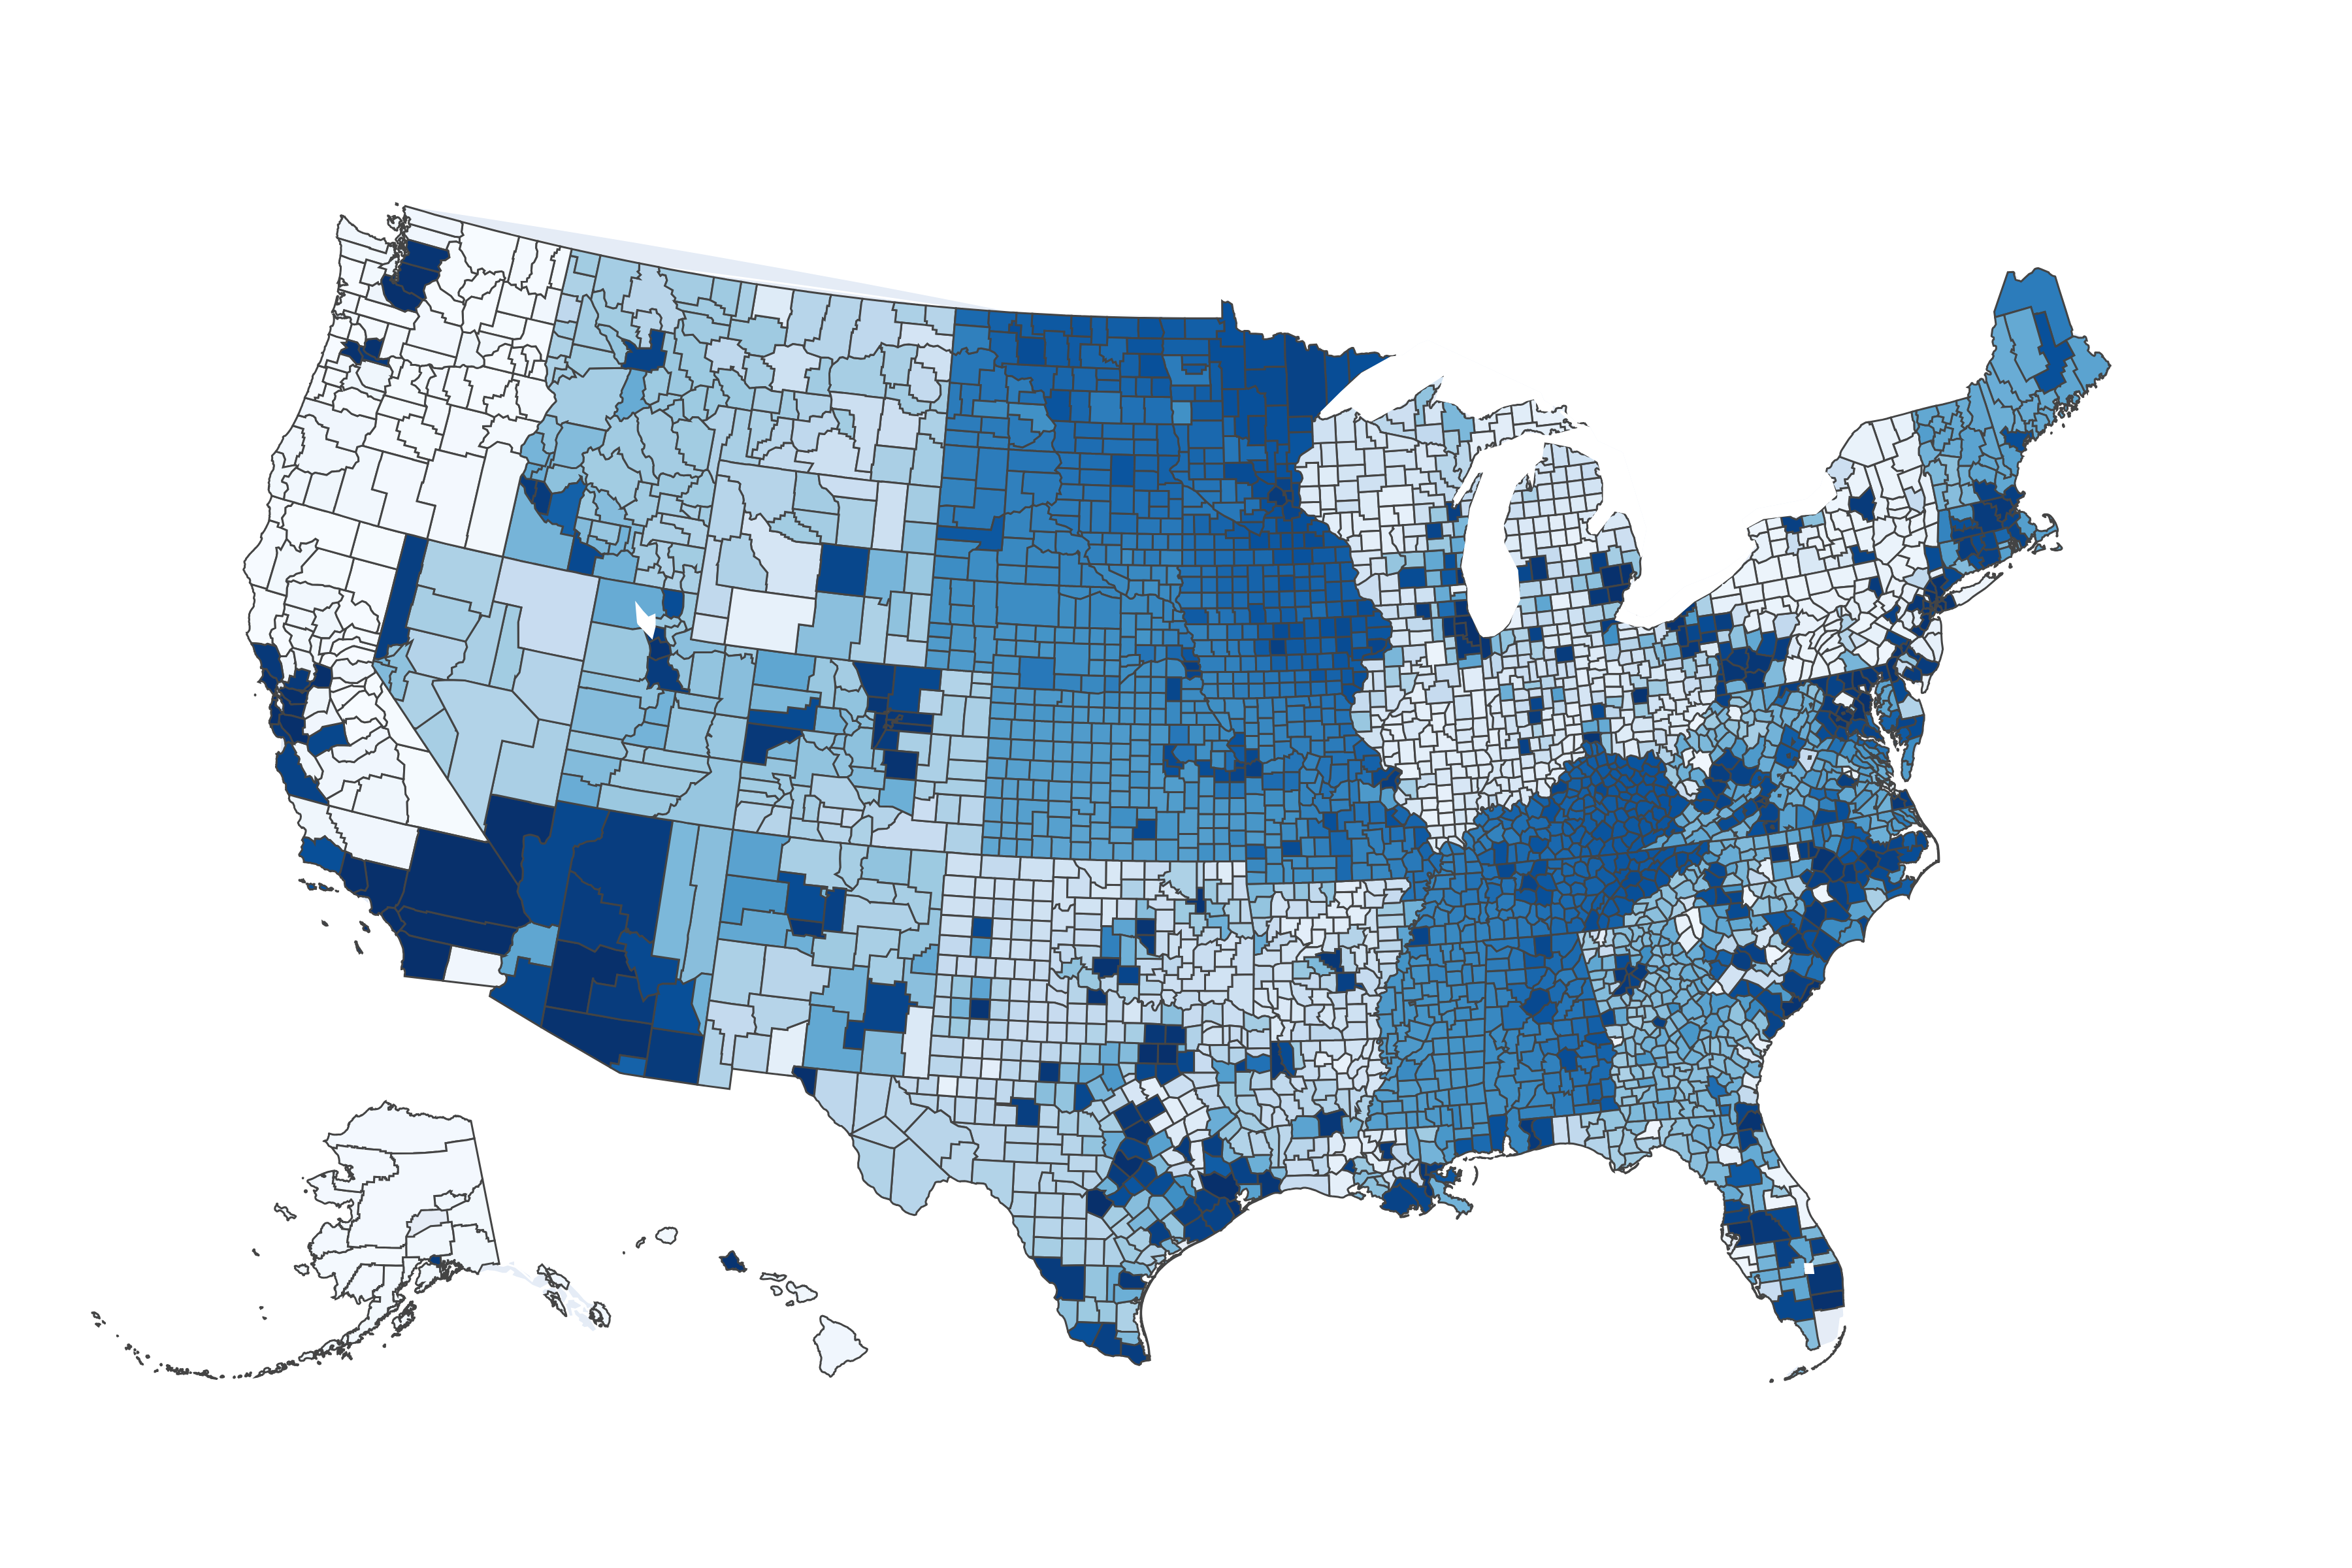
\includegraphics[width=\textwidth]{figures/maps/immigration_shock_2000.png}
        \caption*{\small 1995 - 2000}
    \end{subfigure}
    \hfill
    \begin{subfigure}[b]{\mapwidth}
        \centering
        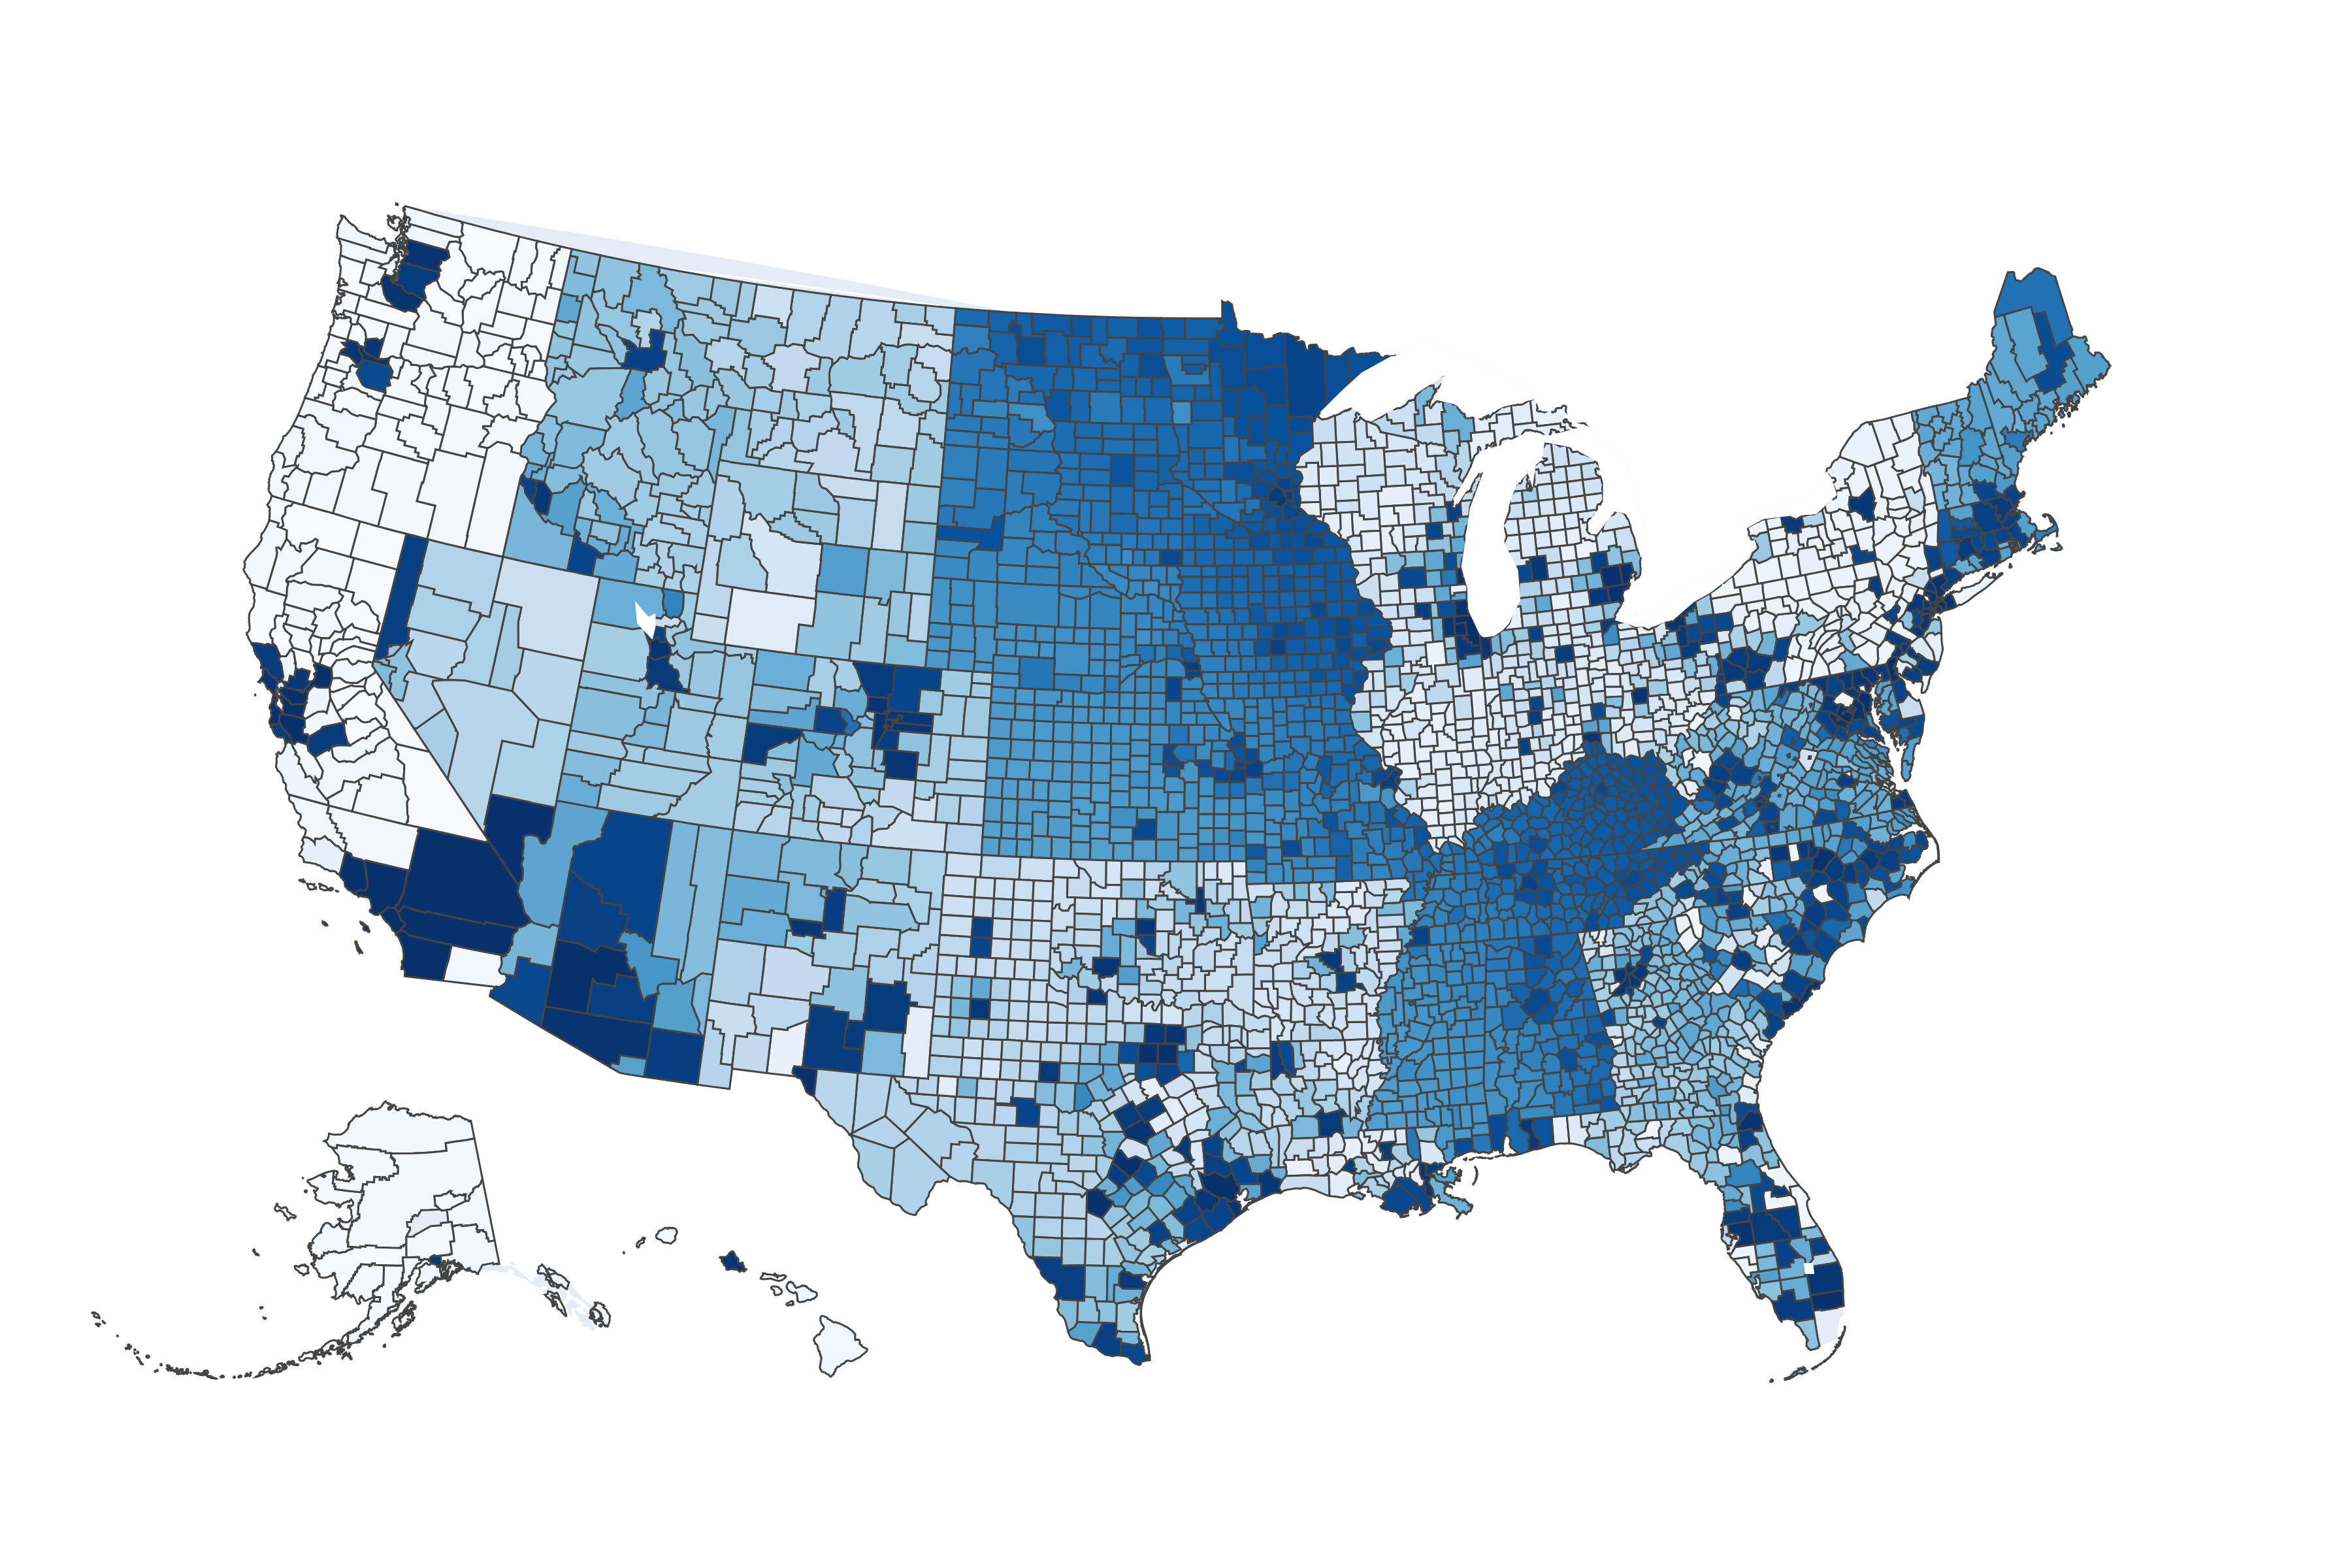
\includegraphics[width=\textwidth]{figures/maps/immigration_shock_2005.png}
        \caption*{\small 2000 - 2005}
    \end{subfigure}
    
    \vspace{0.3em}
    
    % Row 3 (single map, centered)
    \begin{subfigure}[b]{\mapwidth}
        \centering
        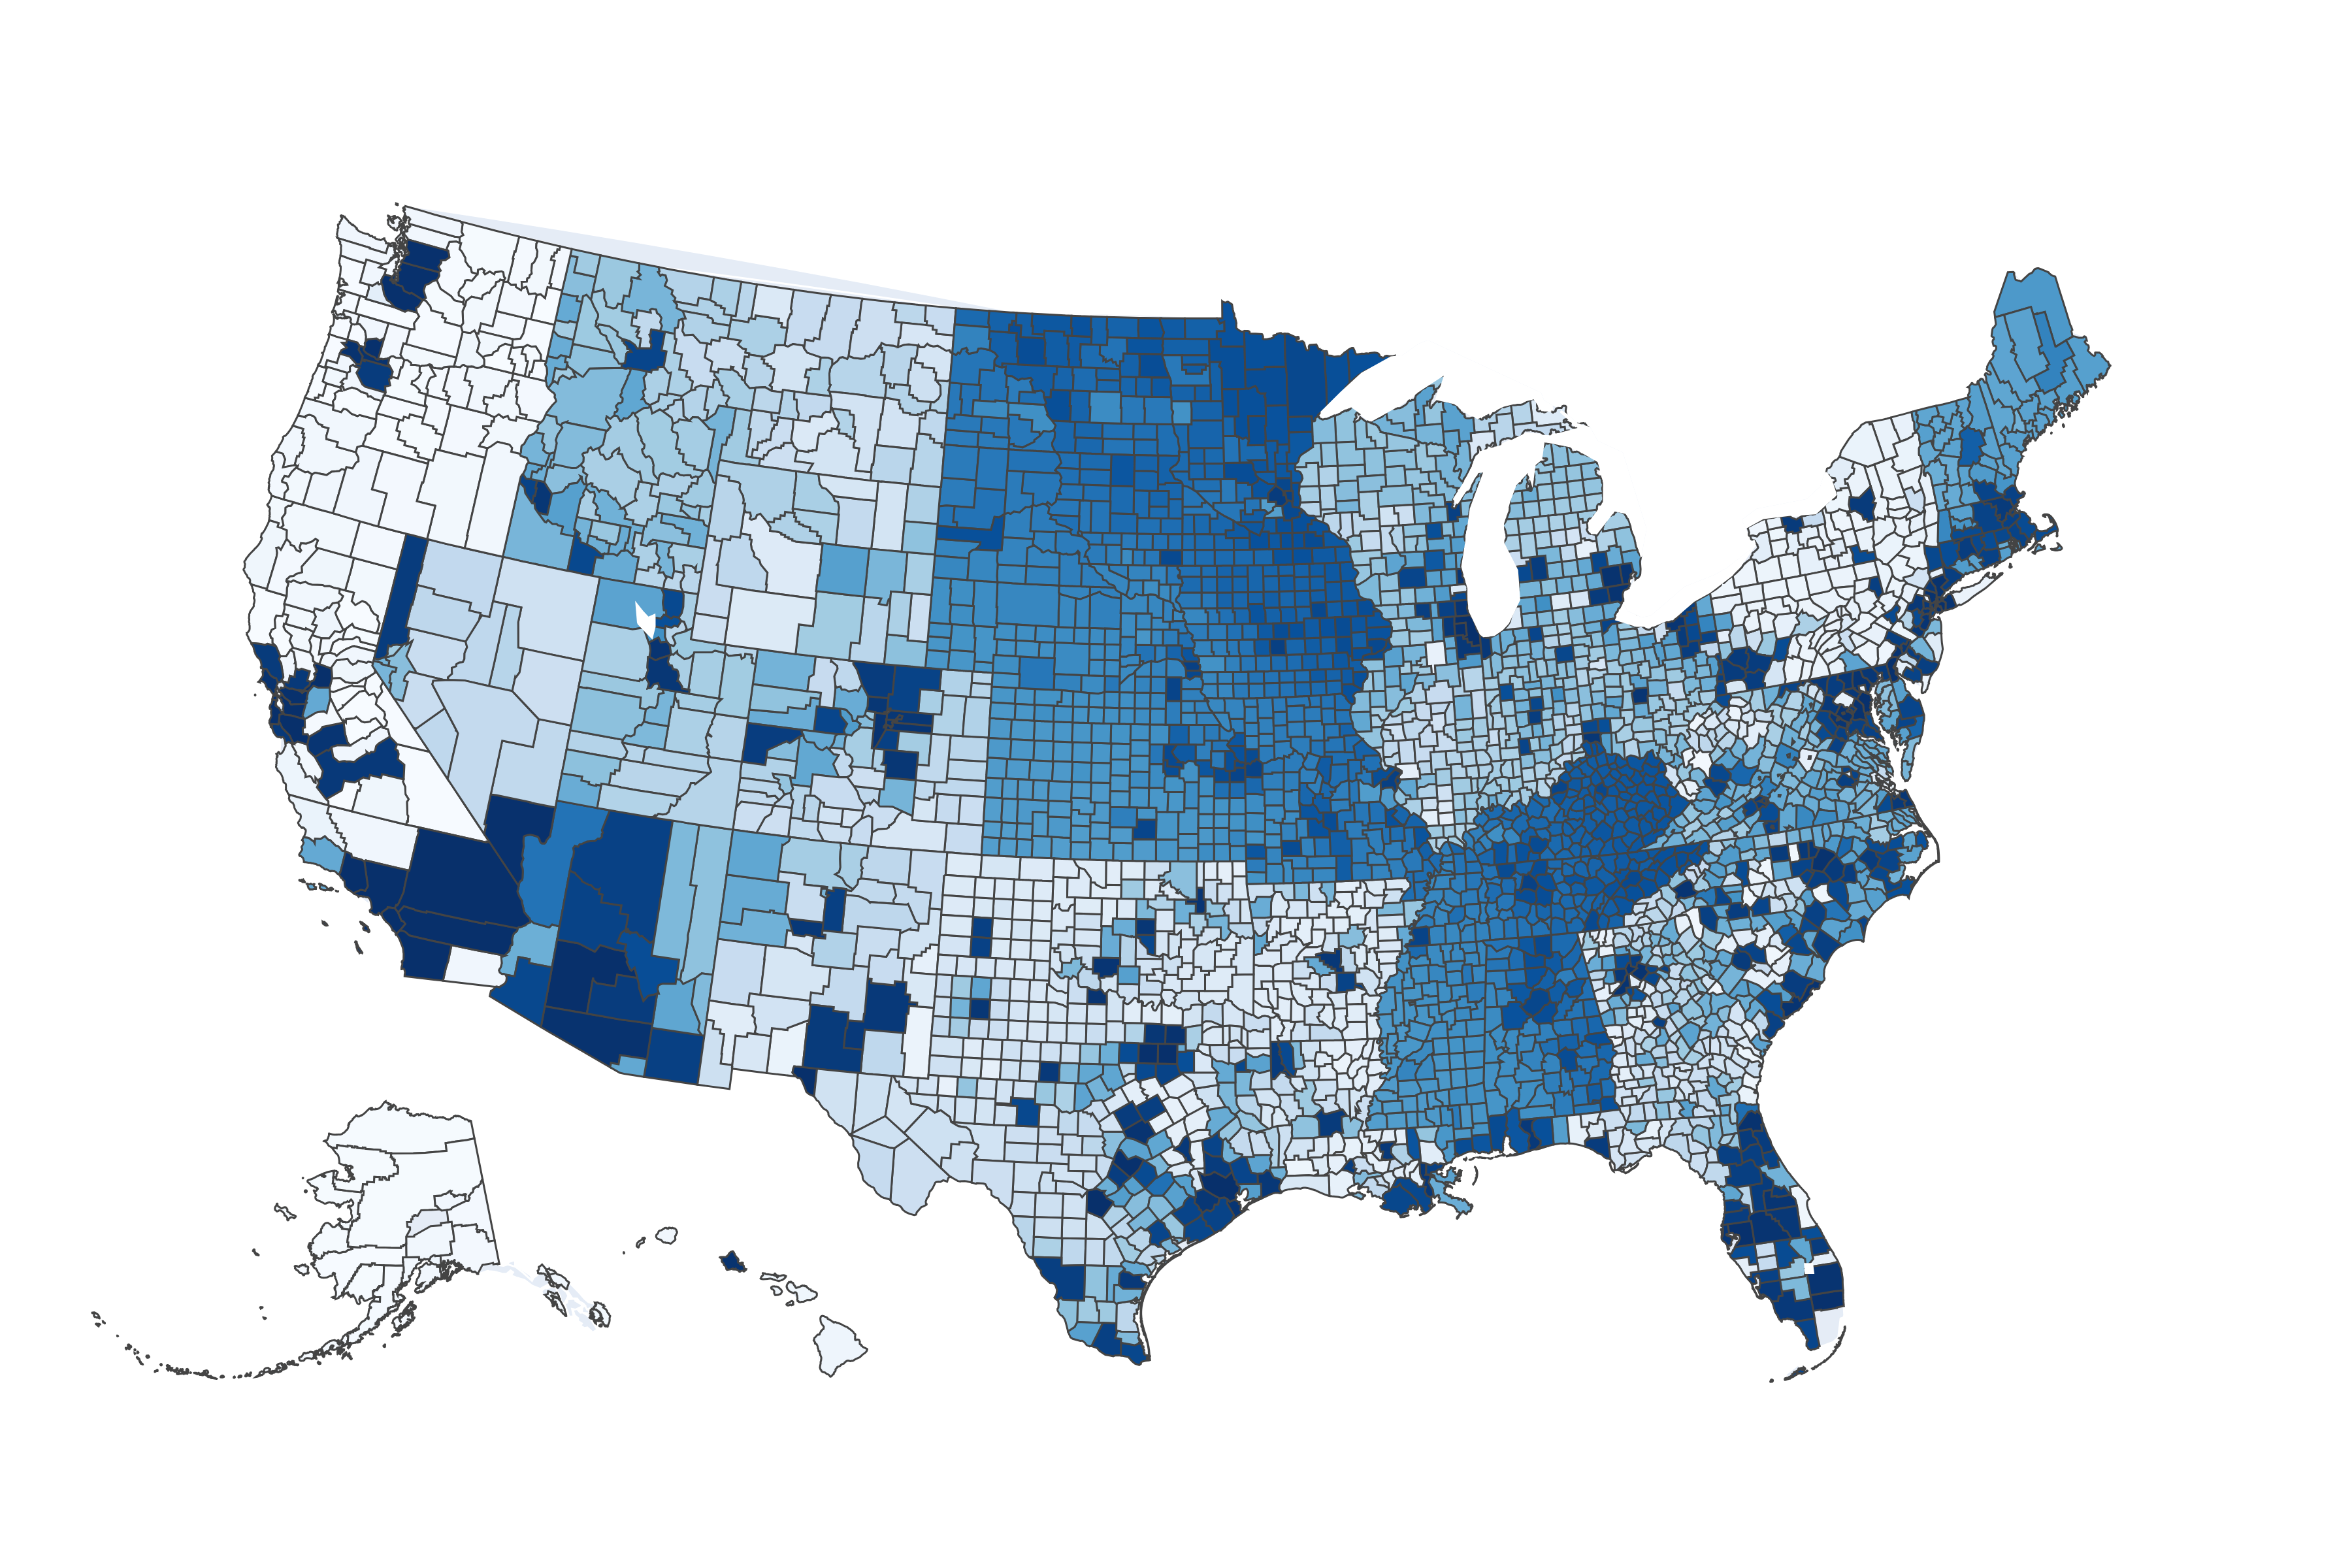
\includegraphics[width=\textwidth]{figures/maps/immigration_shock_2010.png}
        \caption*{\small 2005 - 2010}
    \end{subfigure}
    
    \caption{Immigration Shocks (Instruments) for 5-year periods. The map's color depicts data broken into 200 quantiles with darker colors representing larger values.}
    \label{fig:immigration_map}
\end{figure}